\documentclass{standalone}
\usepackage{tikz}
\usetikzlibrary{patterns, positioning}


\begin{document}
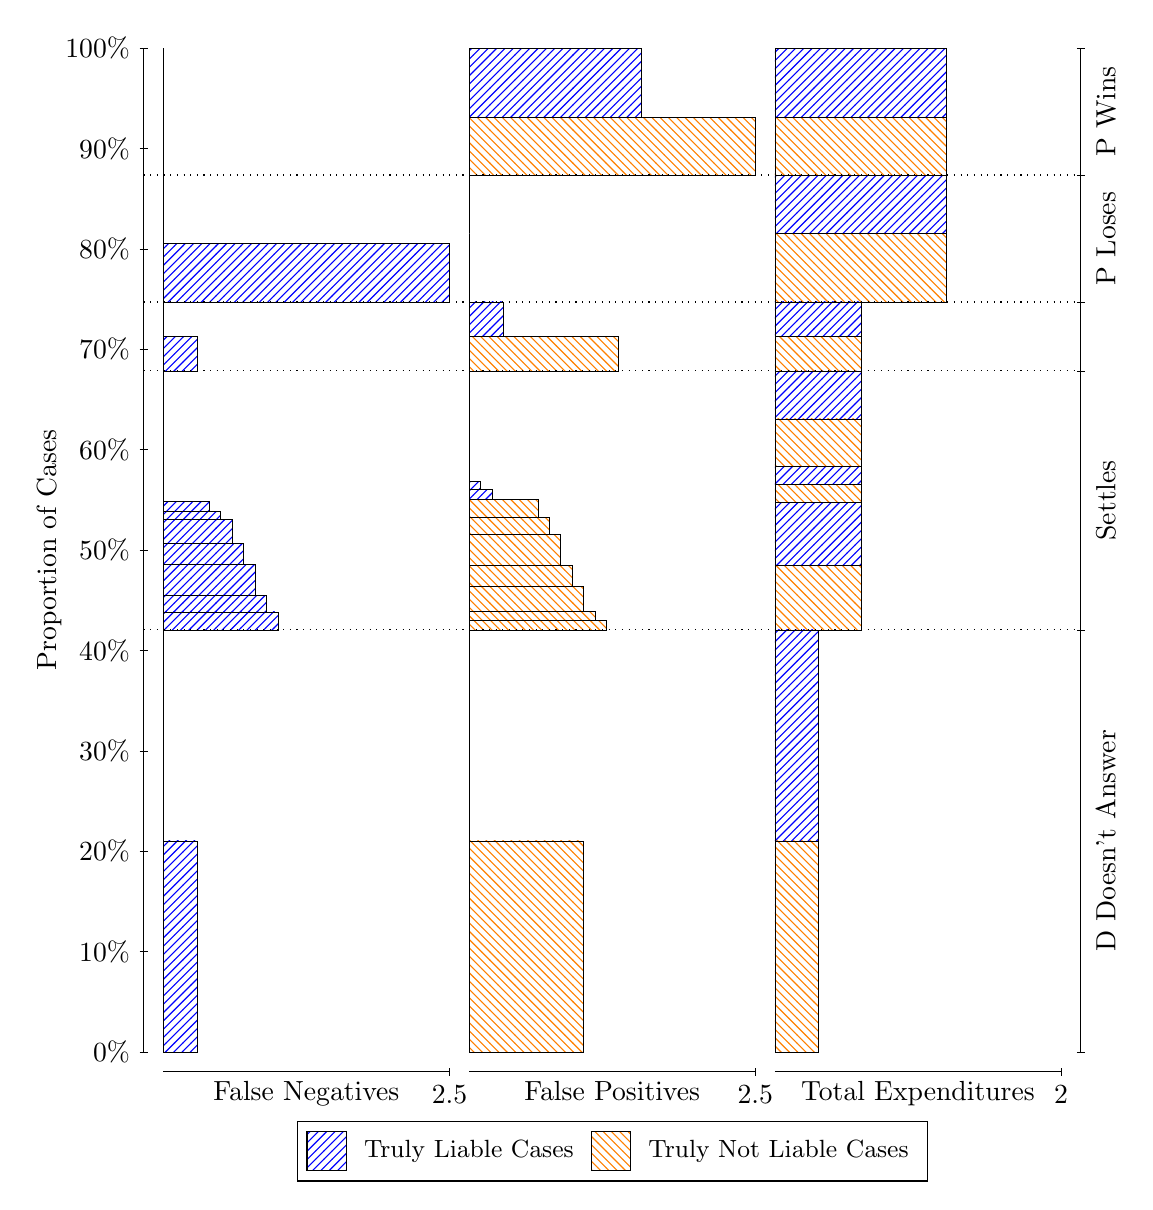
\begin{tikzpicture}
\draw[black, very thin] (1.5,1.75) -- (1.5,14.5);
\node[rotate=90, text=black, anchor=center] at (0.3, 8.125) {Proportion of Cases};
\draw[black, very thin] (1.45,1.75) -- (1.55,1.75);
\node[text=black, anchor=east] at (1.45, 1.75) {0\%};
\draw[black, very thin] (1.45,3.025) -- (1.55,3.025);
\node[text=black, anchor=east] at (1.45, 3.025) {10\%};
\draw[black, very thin] (1.45,4.3) -- (1.55,4.3);
\node[text=black, anchor=east] at (1.45, 4.3) {20\%};
\draw[black, very thin] (1.45,5.575) -- (1.55,5.575);
\node[text=black, anchor=east] at (1.45, 5.575) {30\%};
\draw[black, very thin] (1.45,6.85) -- (1.55,6.85);
\node[text=black, anchor=east] at (1.45, 6.85) {40\%};
\draw[black, very thin] (1.45,8.125) -- (1.55,8.125);
\node[text=black, anchor=east] at (1.45, 8.125) {50\%};
\draw[black, very thin] (1.45,9.4) -- (1.55,9.4);
\node[text=black, anchor=east] at (1.45, 9.4) {60\%};
\draw[black, very thin] (1.45,10.675) -- (1.55,10.675);
\node[text=black, anchor=east] at (1.45, 10.675) {70\%};
\draw[black, very thin] (1.45,11.95) -- (1.55,11.95);
\node[text=black, anchor=east] at (1.45, 11.95) {80\%};
\draw[black, very thin] (1.45,13.225) -- (1.55,13.225);
\node[text=black, anchor=east] at (1.45, 13.225) {90\%};
\draw[black, very thin] (1.45,14.5) -- (1.55,14.5);
\node[text=black, anchor=east] at (1.45, 14.5) {100\%};

\draw[black, very thin] (13.4,1.75) -- (13.4,14.5);
\draw[black, very thin] (13.35,1.75) -- (13.45,1.75);
\node[anchor=west] at (13.35, 1.75) {};
\draw[black, very thin] (13.35,7.1108) -- (13.45,7.1108);
\node[anchor=west] at (13.35, 7.1108) {};
\draw[black, very thin] (13.35,10.4) -- (13.45,10.4);
\node[anchor=west] at (13.35, 10.4) {};
\draw[black, very thin] (13.35,11.275) -- (13.45,11.275);
\node[anchor=west] at (13.35, 11.275) {};
\draw[black, very thin] (13.35,12.887) -- (13.45,12.887);
\node[anchor=west] at (13.35, 12.887) {};
\draw[black, very thin] (13.35,14.5) -- (13.45,14.5);
\node[anchor=west] at (13.35, 14.5) {};

\draw[black, very thin, pattern color=blue, pattern=north east lines] (1.75,1.75) rectangle (2.186,4.4304);
\draw[black, very thin, pattern color=orange, pattern=north west lines] (1.75,4.4304) rectangle (1.75,7.1108);
\draw[black, very thin, pattern color=blue, pattern=north east lines] (1.75,7.1108) rectangle (3.2033,7.3381);
\draw[black, very thin, pattern color=blue, pattern=north east lines] (1.75,7.3381) rectangle (3.058,7.5496);
\draw[black, very thin, pattern color=blue, pattern=north east lines] (1.75,7.5496) rectangle (2.9127,7.9425);
\draw[black, very thin, pattern color=blue, pattern=north east lines] (1.75,7.9425) rectangle (2.7673,8.2119);
\draw[black, very thin, pattern color=blue, pattern=north east lines] (1.75,8.2119) rectangle (2.622,8.5167);
\draw[black, very thin, pattern color=blue, pattern=north east lines] (1.75,8.5167) rectangle (2.4767,8.6183);
\draw[black, very thin, pattern color=blue, pattern=north east lines] (1.75,8.6183) rectangle (2.3313,8.7471);
\draw[black, very thin, pattern color=orange, pattern=north west lines] (1.75,8.7471) rectangle (1.75,10.4);
\draw[black, very thin, pattern color=blue, pattern=north east lines] (1.75,10.4) rectangle (2.186,10.839);
\draw[black, very thin, pattern color=orange, pattern=north west lines] (1.75,10.839) rectangle (1.75,11.275);
\draw[black, very thin, pattern color=blue, pattern=north east lines] (1.75,11.275) rectangle (5.3833,12.019);
\draw[black, very thin, pattern color=orange, pattern=north west lines] (1.75,12.019) rectangle (1.75,12.887);
\draw[black, very thin, pattern color=orange, pattern=north west lines] (1.75,12.887) rectangle (1.75,13.624);
\draw[black, very thin, pattern color=blue, pattern=north east lines] (1.75,13.624) rectangle (1.75,14.5);
\draw[black, very thin, pattern color=orange, pattern=north west lines] (5.6333,1.75) rectangle (7.0867,4.4304);
\draw[black, very thin, pattern color=blue, pattern=north east lines] (5.6333,4.4304) rectangle (5.6333,7.1108);
\draw[black, very thin, pattern color=orange, pattern=north west lines] (5.6333,7.1108) rectangle (7.3773,7.2327);
\draw[black, very thin, pattern color=orange, pattern=north west lines] (5.6333,7.2327) rectangle (7.232,7.3407);
\draw[black, very thin, pattern color=orange, pattern=north west lines] (5.6333,7.3407) rectangle (7.0867,7.6595);
\draw[black, very thin, pattern color=orange, pattern=north west lines] (5.6333,7.6595) rectangle (6.9413,7.9297);
\draw[black, very thin, pattern color=orange, pattern=north west lines] (5.6333,7.9297) rectangle (6.796,8.3238);
\draw[black, very thin, pattern color=orange, pattern=north west lines] (5.6333,8.3238) rectangle (6.6507,8.536);
\draw[black, very thin, pattern color=orange, pattern=north west lines] (5.6333,8.536) rectangle (6.5053,8.764);
\draw[black, very thin, pattern color=blue, pattern=north east lines] (5.6333,8.764) rectangle (5.924,8.8928);
\draw[black, very thin, pattern color=blue, pattern=north east lines] (5.6333,8.8928) rectangle (5.7787,8.9944);
\draw[black, very thin, pattern color=blue, pattern=north east lines] (5.6333,8.9944) rectangle (5.6333,10.4);
\draw[black, very thin, pattern color=orange, pattern=north west lines] (5.6333,10.4) rectangle (7.5227,10.836);
\draw[black, very thin, pattern color=blue, pattern=north east lines] (5.6333,10.836) rectangle (6.0693,11.275);
\draw[black, very thin, pattern color=orange, pattern=north west lines] (5.6333,11.275) rectangle (5.6333,12.143);
\draw[black, very thin, pattern color=blue, pattern=north east lines] (5.6333,12.143) rectangle (5.6333,12.887);
\draw[black, very thin, pattern color=orange, pattern=north west lines] (5.6333,12.887) rectangle (9.2667,13.624);
\draw[black, very thin, pattern color=blue, pattern=north east lines] (5.6333,13.624) rectangle (7.8133,14.5);
\draw[black, very thin, pattern color=orange, pattern=north west lines] (9.5167,1.75) rectangle (10.062,4.4304);
\draw[black, very thin, pattern color=blue, pattern=north east lines] (9.5167,4.4304) rectangle (10.062,7.1108);
\draw[black, very thin, pattern color=orange, pattern=north west lines] (9.5167,7.1108) rectangle (10.607,7.9316);
\draw[black, very thin, pattern color=blue, pattern=north east lines] (9.5167,7.9316) rectangle (10.607,8.7309);
\draw[black, very thin, pattern color=orange, pattern=north west lines] (9.5167,8.7309) rectangle (10.607,8.9589);
\draw[black, very thin, pattern color=blue, pattern=north east lines] (9.5167,8.9589) rectangle (10.607,9.1862);
\draw[black, very thin, pattern color=orange, pattern=north west lines] (9.5167,9.1862) rectangle (10.607,9.7906);
\draw[black, very thin, pattern color=blue, pattern=north east lines] (9.5167,9.7906) rectangle (10.607,10.4);
\draw[black, very thin, pattern color=orange, pattern=north west lines] (9.5167,10.4) rectangle (10.607,10.836);
\draw[black, very thin, pattern color=blue, pattern=north east lines] (9.5167,10.836) rectangle (10.607,11.275);
\draw[black, very thin, pattern color=orange, pattern=north west lines] (9.5167,11.275) rectangle (11.697,12.143);
\draw[black, very thin, pattern color=blue, pattern=north east lines] (9.5167,12.143) rectangle (11.697,12.887);
\draw[black, very thin, pattern color=orange, pattern=north west lines] (9.5167,12.887) rectangle (11.697,13.624);
\draw[black, very thin, pattern color=blue, pattern=north east lines] (9.5167,13.624) rectangle (11.697,14.5);
\draw[black, dotted] (1.5,7.1108) -- (13.4,7.1108);
\draw[black, dotted] (1.5,10.4) -- (13.4,10.4);
\draw[black, dotted] (1.5,11.275) -- (13.4,11.275);
\draw[black, dotted] (1.5,12.887) -- (13.4,12.887);
\draw[black, very thin] (1.75,1.5) -- (5.3833,1.5);
\node[text=black, anchor=north] at (3.5667, 1.5) {False Negatives};
\draw[black, very thin] (5.3833,1.45) -- (5.3833,1.55);
\node[text=black, anchor=north] at (5.3833, 1.45) {2.5};

\draw[black, very thin] (5.6333,1.5) -- (9.2667,1.5);
\node[text=black, anchor=north] at (7.45, 1.5) {False Positives};
\draw[black, very thin] (9.2667,1.45) -- (9.2667,1.55);
\node[text=black, anchor=north] at (9.2667, 1.45) {2.5};

\draw[black, very thin] (9.5167,1.5) -- (13.15,1.5);
\node[text=black, anchor=north] at (11.333, 1.5) {Total Expenditures};
\draw[black, very thin] (13.15,1.45) -- (13.15,1.55);
\node[text=black, anchor=north] at (13.15, 1.45) {2};

\node[text=black, centered, rotate=90] at (13.72, 4.4304) {D Doesn't Answer};
\node[text=black, centered, rotate=90] at (13.72, 8.7555) {Settles};

\node[text=black, centered, rotate=90] at (13.72, 12.081) {P Loses};
\node[text=black, centered, rotate=90] at (13.72, 13.693) {P Wins};

\draw (7.449999999999999,1.5) node[draw=none] (baseCoordinate) {};
\begin{scope}[align=center]
        \matrix[scale=0.5, draw=black, below=0.5cm of baseCoordinate, nodes={draw}, column sep=0.1cm]{
            \node[rectangle, draw, minimum width=0.5cm, minimum height=0.5cm, pattern color=blue, pattern=north east lines] {}; &
            \node[draw=none, font=\small, text=black] (B) {Truly Liable Cases}; &
            \node[rectangle, draw, minimum width=0.5cm, minimum height=0.5cm, pattern color=orange, pattern=north west lines] {}; &
            \node[draw=none, font=\small, text=black] (B) {Truly Not Liable Cases}; \\
            };
\end{scope}

\end{tikzpicture}
\end{document}